\documentclass[tikz]{standalone}
\usepackage{amsmath}
\definecolor{bg}{HTML}{171D2B}
\definecolor{garis}{HTML}{171D2B}
\definecolor{warnaKuning}{HTML}{F7B538}
\definecolor{warnaBiru}{HTML}{4C6EF5}
\definecolor{warnaHijau}{HTML}{40C057}
\definecolor{warnaOranye}{HTML}{E8590C}
\definecolor{warnaMerah}{HTML}{C92A2A}
\definecolor{warnaUngu}{HTML}{BE4BDB}
\definecolor{warnaNavy}{HTML}{1971C2}
\begin{document}
\pagecolor{bg}
\color{white}
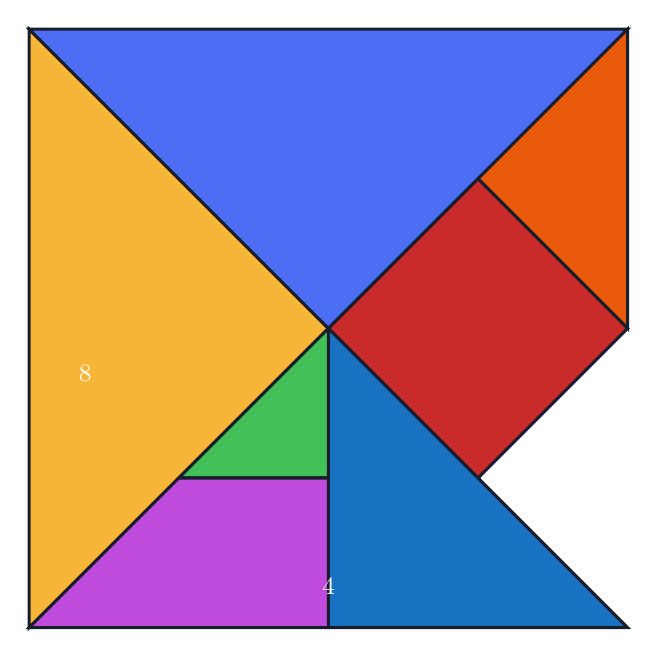
\begin{tikzpicture}[scale=0.95, line width=1.1pt]
  % Tangram klasik dalam persegi 8x8 (koordinat kanonik)
  \filldraw[fill=warnaKuning, draw=garis]  (0,0) -- (0,8) -- (4,4) -- cycle;
  \filldraw[fill=warnaBiru, draw=garis]    (0,8) -- (8,8) -- (4,4) -- cycle;
  \filldraw[fill=warnaHijau, draw=garis]   (2,2) -- (6,2) -- (4,4) -- cycle;
  \filldraw[fill=warnaOranye, draw=garis]  (8,4) -- (8,8) -- (6,6) -- cycle;
  \filldraw[fill=warnaMerah, draw=garis]   (4,4) -- (6,2) -- (8,4) -- (6,6) -- cycle;
  \filldraw[fill=warnaUngu, draw=garis]    (0,0) -- (4,0) -- (6,2) -- (2,2) -- cycle;
  \filldraw[fill=warnaNavy, draw=garis]    (4,0) -- (8,0) -- (4,4) -- cycle;
  % Label sisi kunci
  \node[white, font=\small] at (0.75,3.4) {$8$};
  \node[white, font=\small] at (4.0,0.55) {$4$};
\end{tikzpicture}
\end{document}
